\newcommand*{\orawidest}{accept}
\newcommand*{\oratallest}{\#\#}
\newlength{\orawidth}
\settowidth{\orawidth}{\orawidest}
\newcommand*{\ora}[1]{\overrightarrow{#1\vphantom{\oratallest}}}
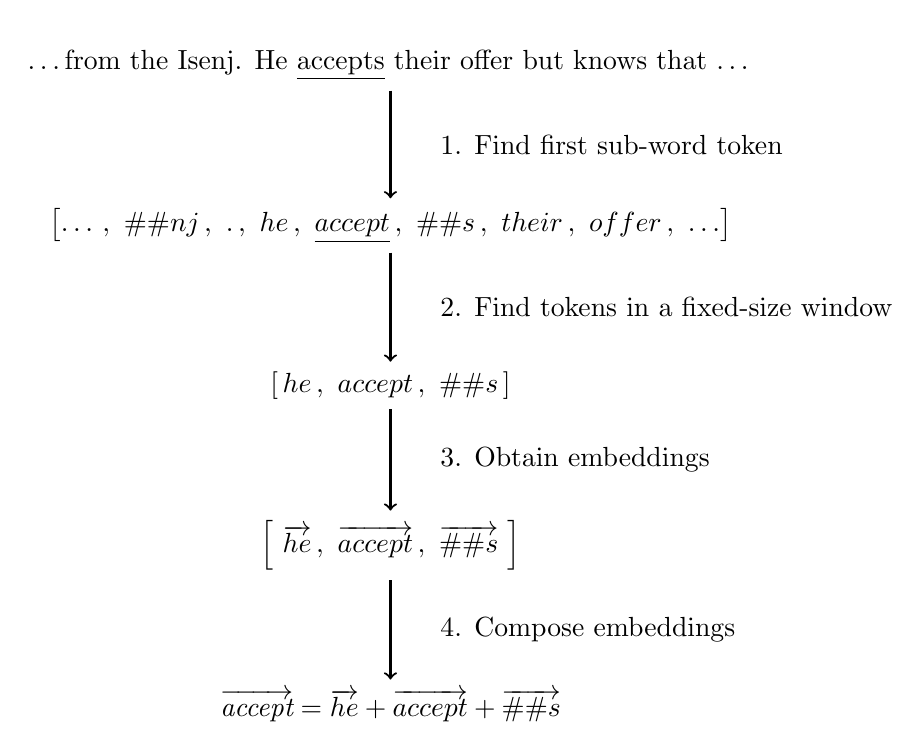
\begin{tikzpicture}[
    every path/.style = {thick, ->},
    every node/.style = {inner sep = 0, outer sep = 0.05in},
    node distance = 0.8in
  ]
  \node [label] (a) {\dots from the Isenj. He \underline{accepts} their offer but knows that \dots };
  \node [label, below of=a] (b) {$\left[ \dots\,,\ \text{\#\#nj}\,,\ .\,,\ \text{he}\,,\ \text{\underline{accept}}\,,\ \text{\#\#s}\,,\ \text{their}\,,\ \text{offer}\,,\ \dots \right]$};
  \node [label, below of=b] (c) {$\left[ \, \text{he}\,,\ \text{accept}\,,\ \text{\#\#s} \, \right]$};
  \node [label, below of=c] (d) {$\left[ \ \ora{\text{he}}\,,\ \ora{\text{accept}}\,,\ \ora{\text{\#\#s}} \ \right]$};
  \node [label, below of=d] (e) {$ \ora{\textit{accept}} = \ora{\text{he}} + \ora{\text{accept}} + \ora{\text{\#\#s}}$};
  \draw (a) -- (b) node[midway, right=0.2in] {1. Find first sub-word token};
  \draw (b) -- (c) node[midway, right=0.2in] {2. Find tokens in a fixed-size window};
  \draw (c) -- (d) node[midway, right=0.2in] {3. Obtain embeddings};
  \draw (d) -- (e) node[midway, right=0.2in] {4. Compose embeddings};
\end{tikzpicture}